\begin{enumerate}[label=\thechapter.\arabic*,ref=\thechapter.\theenumi]
\item Let y\brak{t}=x\brak{4t},where x\brak{t} is a continous-time periodic signal of $100$s.the fundamental period of y\brak{t} is (\textbf{rounded off to the nearest integer})
 \hfill(GATE IN 2023)\\
\solution

\item
In the circuit shown below, the amplitudes of the voltage across the resistor and the capacitor are equal. What is the value of the angular frequency $\omega_o$ (in rad/s)? 
(Round off the answer to one decimal place.)
\begin{figure}[ht]
    \centering
    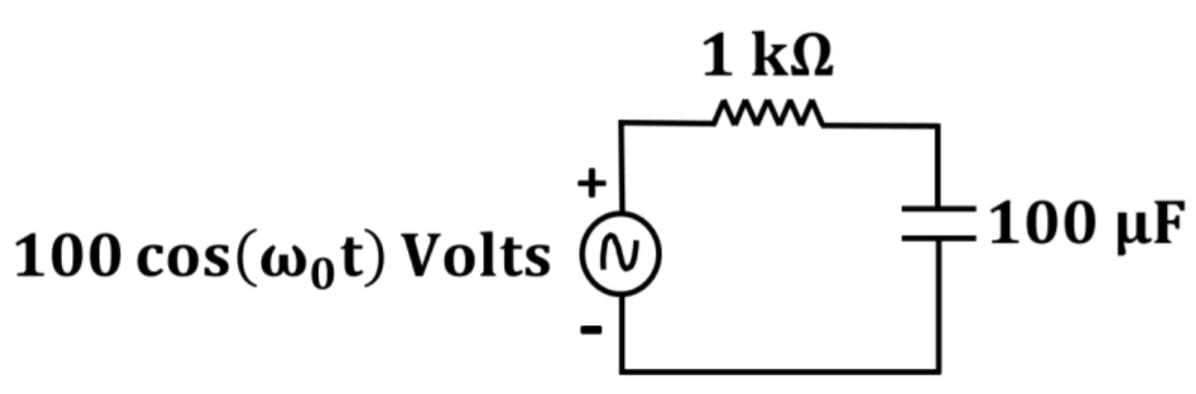
\includegraphics[width = 8cm]{2023/BM/32/figs/fig1.jpg}
    \label{fig:BM_32}
\end{figure}\hfill(GATE 23 BM Q32)\\
\solution

\end{enumerate}
